% !TEX root = /home/fred-olav/afgv/src/preamble.tex
\input preamble.tex

\centerline{\bf Lekseprøve i PLS IO koblinger}  \bigskip

Oppgave 1

To endebrytere skal tilkobles h.h.v. \texttt{Ix.5} og \texttt{Ix.11} på en Siemens SM-321 DI inngangsmodul.(model 6ES7321-1BL00-0AA0) Tegn de nødvendige koblingene. Det internekoblingsskjemaet for (\texttt{Ix.0}) vises som en referanse for alle inngangene.
Tegn de nødvendige koblingene som er nødvendig for tilkobling av endebryterene.  


$$\includegraphics[width=15.5cm]{aPLS_IO_YFFx01.eps}$$

Er dette en \textit{sinking} eller en \textit{sourcing} DI modul?
Tegn strømretning på alle ledere til IO-modulen. 
\vfil
\eject 
Oppgave 2


Tegn de nødvendige koblingene for å tilkoble en relespole til den digitale utgangen \texttt{Y3} på en Koyo "CLICK" PLS model C0-00DD1-D. Det interne skjemaet for den første utgangen vises som en referanse for alle (\texttt{Y2} til \texttt{Y4}). 


$$\includegraphics[width=15.5cm]{aPLS_IO_YFFx02.eps}$$

Avgjør om dette er en \textit{sinking} eller en \textit{sourcing} PLS utgang. 
\eject
Oppgave 3


%Tegn inn de nødvendige koblingene for å koble to trykkbrytere og to relespoler til en Allen-Bradley MicroLogix 1000 PLC(model 1761-L10BWA, med 6 DI-er som enten er sourcing eller sinking, og 4 DO med potensialfrie kontakter.) Være nøye med å koble bryterene sånn at di \textit{source} til PLS inngangene. (Prassure Switch Low til \texttt{I/2} og Preassure Switch High til \texttt{I/5}. Begge bruker Normalt Open  kontakten. Koble relespolene slir at PLS-en \textit{source}strøµ til de.(\texttt{O/0} og \texttt{O/1}):


\vskip 50pt

$$\includegraphics[width=10.5cm]{aPLS_IO_YFFx03.eps}$$

\end {document}
